% vim: set textwidth=78 autoindent:

\subsection{OGR-Layer-Konverter Plugin}

% when the revision of a section has been finalized, 
% comment out the following line:
%\updatedisclaimer

Das Plugin \toolbtntwo{ogr_converter}{OGR-Layer-Konverter} erm�glicht es,
Vektorlayer von einem OGR-unterst�tzten Vektorformat in ein anderes
OGR-unterst�tztes Vektorformat zu konvertieren. Es ist sehr einfach zu
verwenden und bietet Funktionalit�ten wie in Abbildung
\ref{fig:ogrconverter_dialog} dargestellt. Die unterst�tzten Vektorformate
k�nnen je nach GDAL Installation unterschiedlich sein.

\begin{itemize}
\item \textbf{Quelle Format/Datensatz/Layer}: Geben Sie das OGR-Format und
den Datensatz der konvertiert werden soll an.
\item \textbf{Ziel Format/Datensatz/Layer}: Geben Sie das OGR-Format und die
Vektor Ausgabedatei an.
\end{itemize}

\begin{figure}[ht]
   \begin{center}
   \caption{OGR-Layer-Konverter Plugin \nixcaption}\label{fig:ogrconverter_dialog}\smallskip
   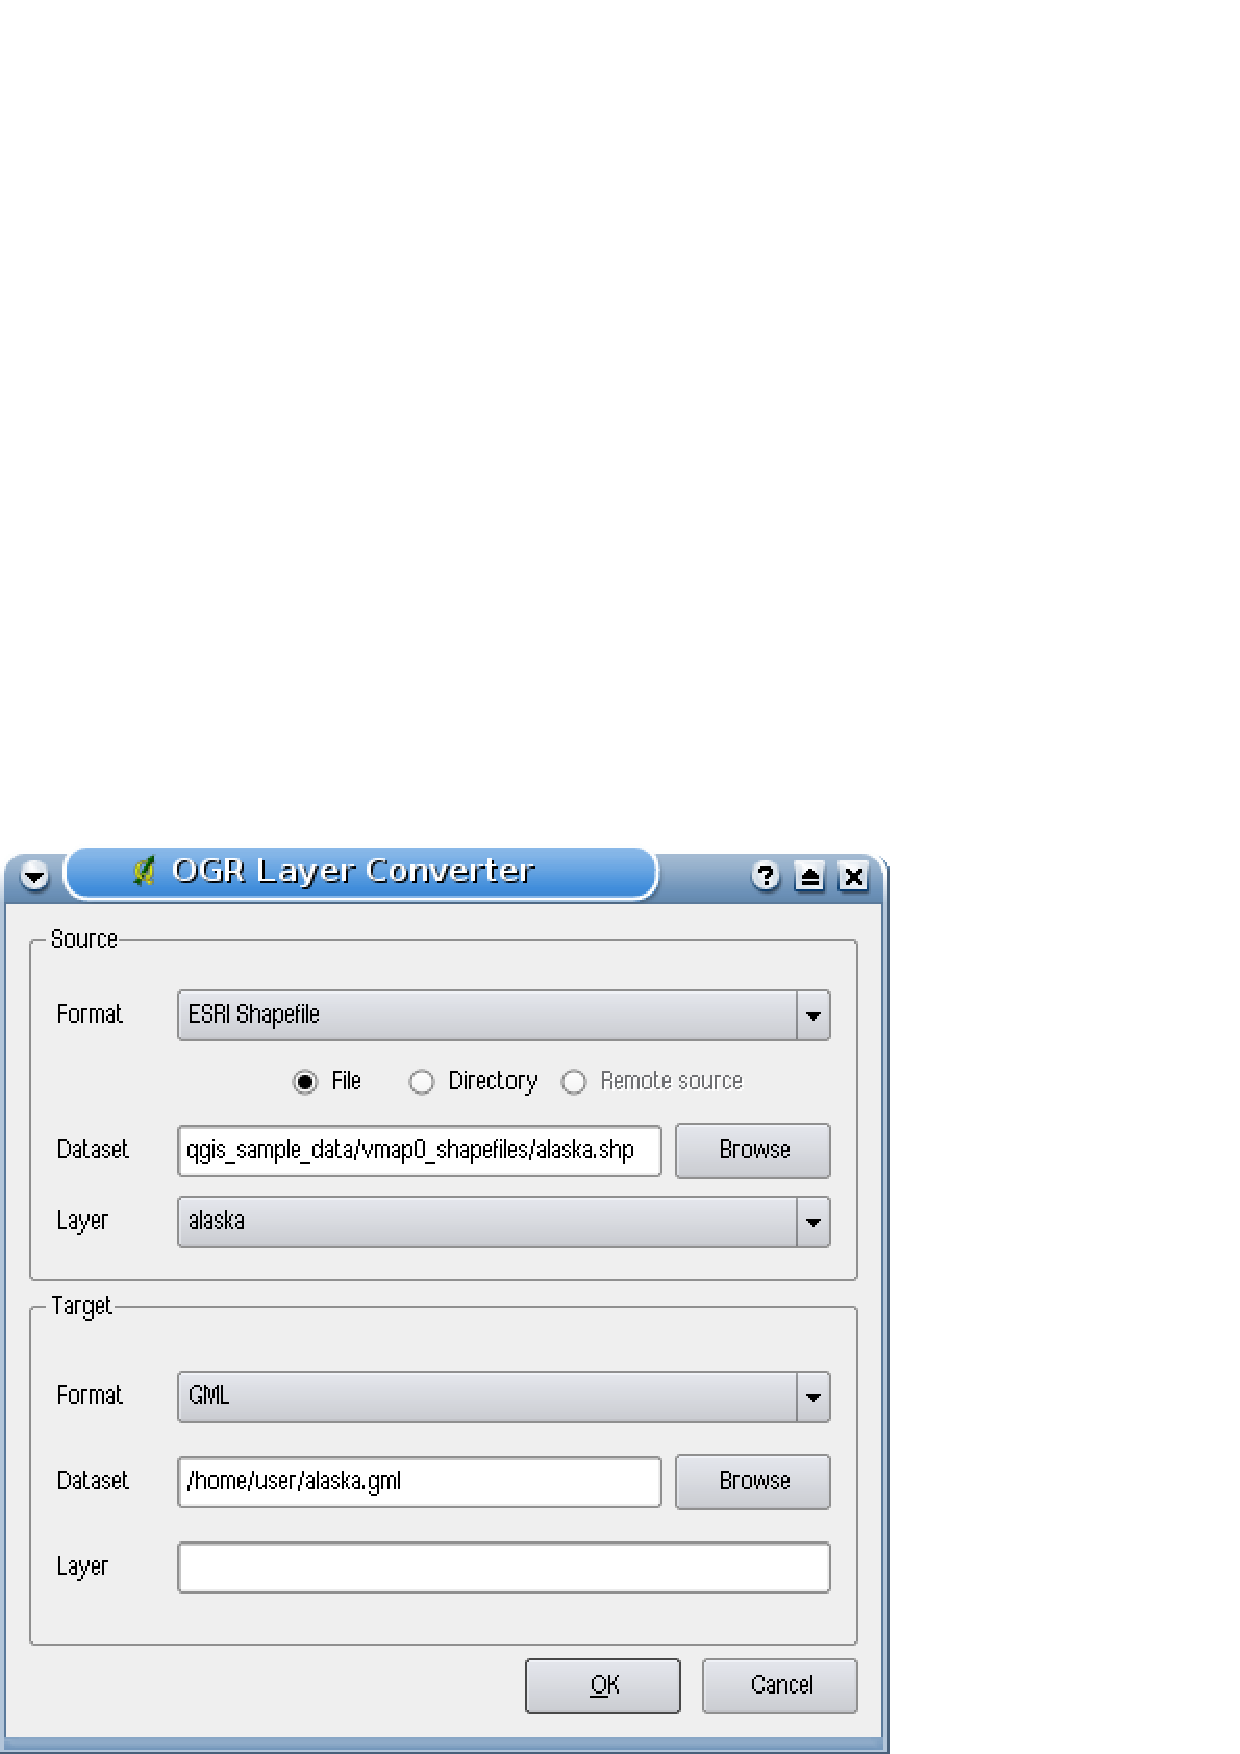
\includegraphics[clip=true, width=9cm]{ogrconverter_dialog}
\end{center}  
\end{figure}

\begin{enumerate}
  \item Starten Sie QGIS, laden Sie das OGR-Konverter Plugin mit dem Plugin
Manager (siehe Kapitel~\ref{sec:load_core_plugin}) und klicken Sie auf das
neue Icon \toolbtntwo{ogr_converter}{OGR Layer Converter} in der
Werkzeugleiste. Der Dialog \dialog{OGR-Layer-Konverter} erscheint wie in
Abbildung~\ref{fig:ogrconverter_dialog}.
  \item W�hlen Sie als OGR-unterst�tztes Vektorformat \selectstring{ESRI
Shapefile}{} und als Datensatz \filename{alaska.shp} im Bereich Quelle.
  \item W�hlen Sie als OGR-unterst�tztes Vektorformat \selectstring{GML}{}
und als Ausgabe \filename{alaska.gml} im Bereich Ziel.
  \item Klicken Sie auf \button{Ok}.
\end{enumerate}

\newpage


